\documentclass[11pt,a4paper,english]{article}
    \usepackage[latin1]{inputenc}
    \usepackage{amsmath,amsfonts,amssymb}
    \usepackage{enumitem}
    \usepackage{fullpage}
    \usepackage{graphicx}
    \usepackage{tabto}
    \usepackage{etoolbox}
    \usepackage{xcolor}
    \usepackage{hyperref}
    \usepackage{minted}
    \usepackage{parskip}
    \usepackage[title]{appendix}
    \usepackage[font=small,labelfont=bf]{caption}
    \hypersetup{ colorlinks = true}
    \graphicspath{ {./} }

    \title{Bayesian Data Analysis - Assignment 6}
    \author{}

    \begin{document}
        \maketitle
      \definecolor{bg}{rgb}{0.95,0.95,0.95}

      This exercise was implemented using $pystan$ and $python$. This is how the $Stan$ model look like:
      \begin{minted}[bgcolor=bg,fontsize=\small,autogobble]{python}
        data {
          int<lower=0> total;
          int<lower=0> deaths[total];
          int<lower=0> numb_of_animals[total];
          vector[total] doses;
          vector[2] mu;
          cov_matrix[2] cov_m;
        }
        parameters {
            vector[2] alpha_beta;
        }
        model {
            alpha_beta ~ multi_normal(mu, cov_m);
            deaths ~ binomial_logit(numb_of_animals, alpha_beta[1] + alpha_beta[2] * doses);
        }
      \end{minted}

      Total of \textbf{5} chains with \textbf{50,000} samples were generated, from which \textbf{5000} "burn-in"s were removed.
      \begin{minted}[bgcolor=bg,fontsize=\small,autogobble]{python}
        fit = stan_model.sampling(data=data, iter=10000, warmup=1000, chains=5)
      \end{minted}

      The \textbf{$\widehat{R}$ values} in my case are:

      \begin{align*}
        \widehat{R}_{\alpha} = 1.0 \\
        \widehat{R}_{\beta} = 1.0
      \end{align*}

      \begin{minted}[bgcolor=bg,linenos,fontsize=\small,autogobble]{python}
                        mean   se_mean   sd   2.5%    25%    50%    75%  97.5%  n_eff   Rhat
        alpha_beta[1]   0.99    0.03    0.9  -0.62   0.37   0.91   1.57   2.78    813    1.0
        alpha_beta[2]  10.67    0.17   4.69   3.39   7.19  10.08   13.5  21.29    783    1.0
      \end{minted}

      The \textbf{interpretation of Rhat values}: As both $\widehat{R}_{\alpha}$ and $\widehat{R}_{\beta}$ values are $1.0$, which is below $1.01$, that \textbf{means that the generated chains are well converged}.

      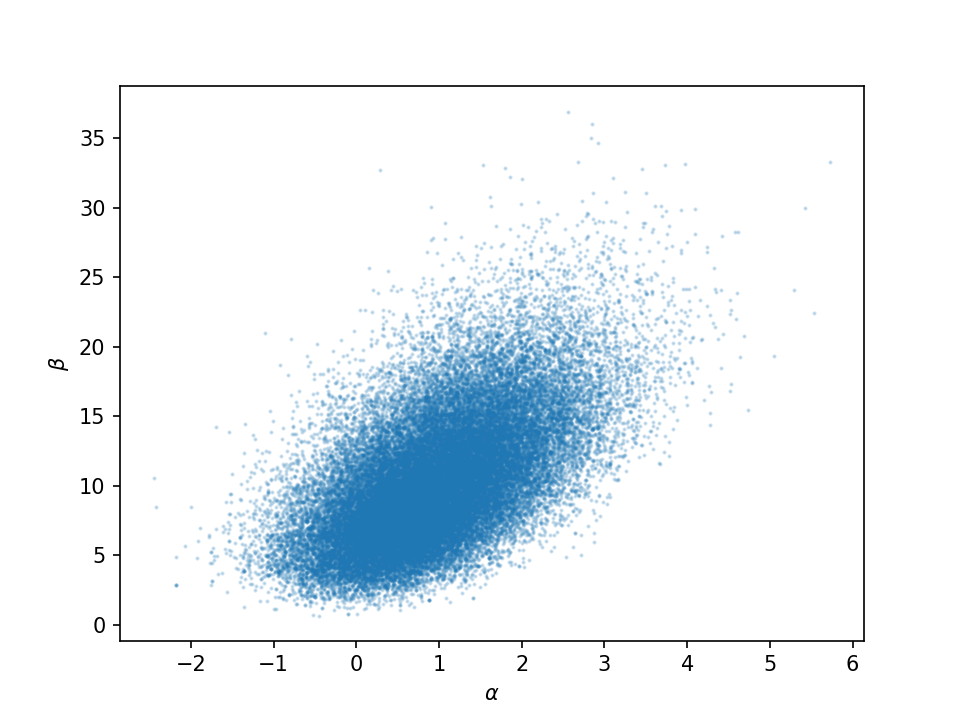
\includegraphics[width=17.7cm]{scatter.png}
      \captionof{figure}{A plot of 5 chains with 50,000 iterations and 5,000 warmup.}

      \begin{appendices}
        \section{Source code}
        \begin{minted}[bgcolor=bg,linenos,fontsize=\small,autogobble]{python}
            import matplotlib
            matplotlib.use('TkAgg')
            import matplotlib.pyplot as plt
            import numpy as np

            import pystan

            # Init all the params based on the description
            sigma_a = 2
            sigma_b = 10
            mu_a = 0
            mu_b = 10
            cor = 0.5
            cov_matrix = np.array([
                [sigma_a**2,                cor * sigma_a * sigma_b],
                [cor * sigma_a * sigma_b,   sigma_b**2]
            ])
            mean = np.array([mu_a, mu_b])

            doses = np.array([-0.86, -0.3, -0.05, 0.72])
            deaths = np.array([0, 1, 3, 5])
            number_of_animals = np.array([5, 5, 5, 5])

            # stan code
            stan_code = '''
            data {
                int<lower=0> total;
                int<lower=0> deaths[total];
                int<lower=0> numb_of_animals[total];
                vector[total] doses;
                vector[2] mu;
                cov_matrix[2] cov_m;
            }
            parameters {
                vector[2] alpha_beta;
            }
            model {
                alpha_beta ~ multi_normal(mu, cov_m);
                deaths ~ binomial_logit(numb_of_animals, alpha_beta[1] + alpha_beta[2] * doses);
            }
            '''

            # calculation code
            stan_model = pystan.StanModel(model_code=stan_code)
            data = dict(
                total=len(number_of_animals),
                deaths=deaths,
                numb_of_animals=number_of_animals,
                doses=doses,
                mu=mean,
                cov_m=cov_matrix,
            )
            fit = stan_model.sampling(data=data, iter=10000, warmup=1000, chains=5)
            print(fit)

            # graph
            extracted_samples = fit.extract(permuted=True)
            samples = extracted_samples['alpha_beta']
            plt.scatter(samples[:, 0], samples[:, 1], s=1.4, alpha=0.3)
            plt.ylabel(r'$\beta$')
            plt.xlabel(r'$\alpha$')
            plt.savefig('./ex6/report/scatter.png')

            # output
            '''
                            mean se_mean     sd   2.5%    25%    50%    75%  97.5%  n_eff   Rhat
            alpha_beta[1]   0.99    0.03    0.9  -0.62   0.37   0.91   1.57   2.78    813    1.0
            alpha_beta[2]  10.67    0.17   4.69   3.39   7.19  10.08   13.5  21.29    783    1.0
            '''
        \end{minted}
      \end{appendices}
  \end{document}
